
Consider a two-dimensional lattice of $N\times N$ spins. 
Every spin can take values $s_{i,j}=\pm1$ and the system 
is governed by the Hamiltonian
\begin{equation}
    \mathcal{H}=-J\cdot\sum_{NN}s_{i,j}s_{k,l}
\end{equation}
with $J$ being the interaction strength. The sum is only 
over nearest neighbors (NN), meaning that the spin 
$s_{i,j}$ at $x=i,y=j$ interacts only with spins at 
$s_{i\pm1,j}$ and $s_{i,j\pm1}$. Assume periodic boundary
conditions in both directions, meaning that, for instance, 
spin $s_{0,j}$ interacts with $s_{1,j}$ and with 
$s_{N-1,j}$ on "the other side". In the following, put 
$J=1$ and $k_B=1$ for simplicity.

\paragraph{1. Write a code (and submit it along with your 
    results) that implements the following algorithm
    (called "importance sampling with the Metropolis 
    algorithm")
} \ \\

\begin{itemize}
    \item Initialize the spins with $s=\pm1$ randomly 
        chosen in an $N\times N$ array. \\
        \lstinputlisting[firstline=16,lastline=23]{./code/main.py}
    \item Pick a spin $(i,j)$ at random. Calculate the 
        energy change $\delta E$ upon flipping only this 
        spin $(i,j)$. If $\delta E<0$, accept the spin 
        flip. If $\delta E>0$, accept the flip with 
        Boltzmann probability $\exp(-\beta\delta E)$, 
        otherwise reject. \\
        \lstinputlisting[firstline=52,lastline=72]{./code/main.py} \ \\
        \newpage
        Here, the flip energy is given by
        \lstinputlisting[firstline=26,lastline=50]{./code/main.py}

    \item After every $N^2$ of such spin "tests", 
        evaluate the mean magnetization 
        $\langle M\rangle=\frac{1}{N^2}\sum_{i,j}s_{i,j}$
        (note that the sum here is over all spins) \\
        \\
        Get the magnetization for a given grid:
        \lstinputlisting[firstline=74,lastline=82]{./code/main.py}
        \newpage
        Calculate mean magnetization after every $N^2$ "tests",
        do this for different temperatures and plot.
        \lstinputlisting[firstline=114,lastline=136]{./code/main.py} \ \\
        Plotting is done with this function: 
        \lstinputlisting[firstline=85,lastline=111]{./code/main.py} 

    % \newpage
    \item Why does this simple method sample phase 
        space (rather) efficiently? \\
        \\
        Choosing spins at random is an unbiased way of 
        doing the calculation, since all grid cells are 
        equally important. 
\end{itemize}

\paragraph{2. Study the system numerically for $N=32$ or 
    higher and for the two temperatures $T=3$ and $T=1.5$ 
    (note again that $J=1=k_B$, hence $T$ is the only 
    parameter). Continue running the algorithm, until 
    $\langle M\rangle$ does not change anymore except for 
    small fluctuations around a constant value. Discuss 
    your results.
    % If you are more ambitious, you may wish to measure a full curve ⟨M⟩(T) for temperatures in
} \ \\
    \\
    The code above leads to the creation of the following
    plot.
    \begin{figure}[h!]
        \centering
        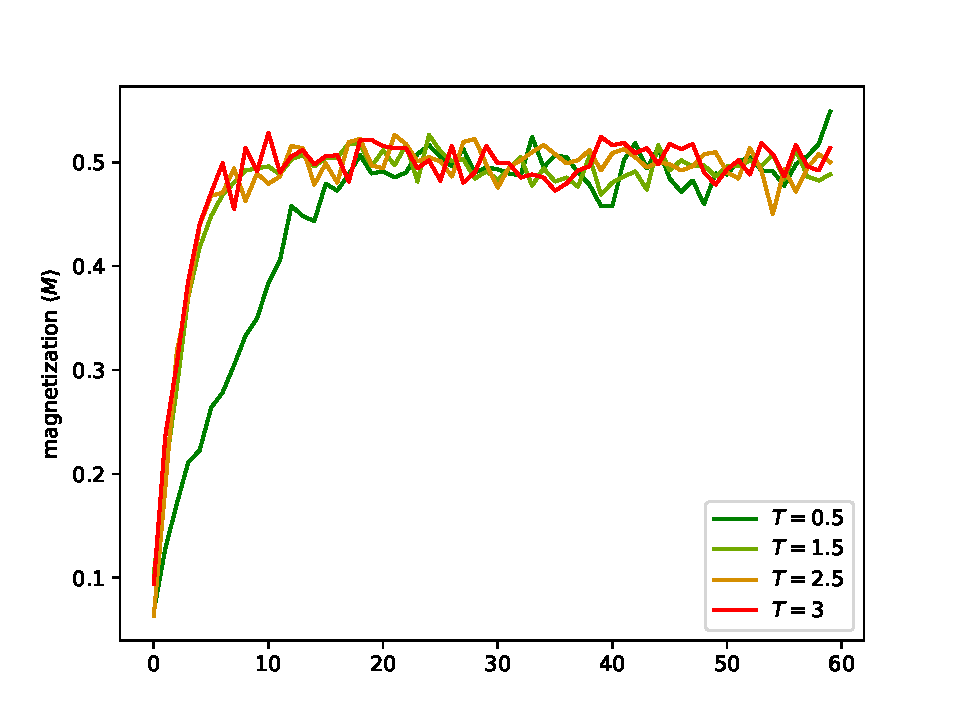
\includegraphics[width=.7\textwidth]{./figures/magnetization_vs_time.pdf}
    \end{figure} \ \\ 
    From this we can verify a few expectations.
    \begin{enumerate}
        \item The state of least energy is one where all 
            spins align. The system tends toward
            this state over time. 
        \item Whether all spins align to be $+1$ or $-1$ 
            is arbitrary and can change from run to run,
            since it depends both on the random 
            initialization as well as the randomness 
            in the flip probability calculations.
        \item For higher temperatures, spins might flip 
            with a non-zero probability even if the 
            energy change is positive. For this reason, 
            one can see in the plot that the system at 
            $T=3$ approximates the low-energy state a bit
            more slowly than the system at $T=1.5$ does.
    \end{enumerate}
    
    \newpage
    Visualization of the grid's state at various times.
    \begin{figure}[h!]
        \centering
        \begin{minipage}{.5\linewidth}
          \centering
          \subfloat[spins for $T=1.5$ after initialization]{
            \label{:a}
            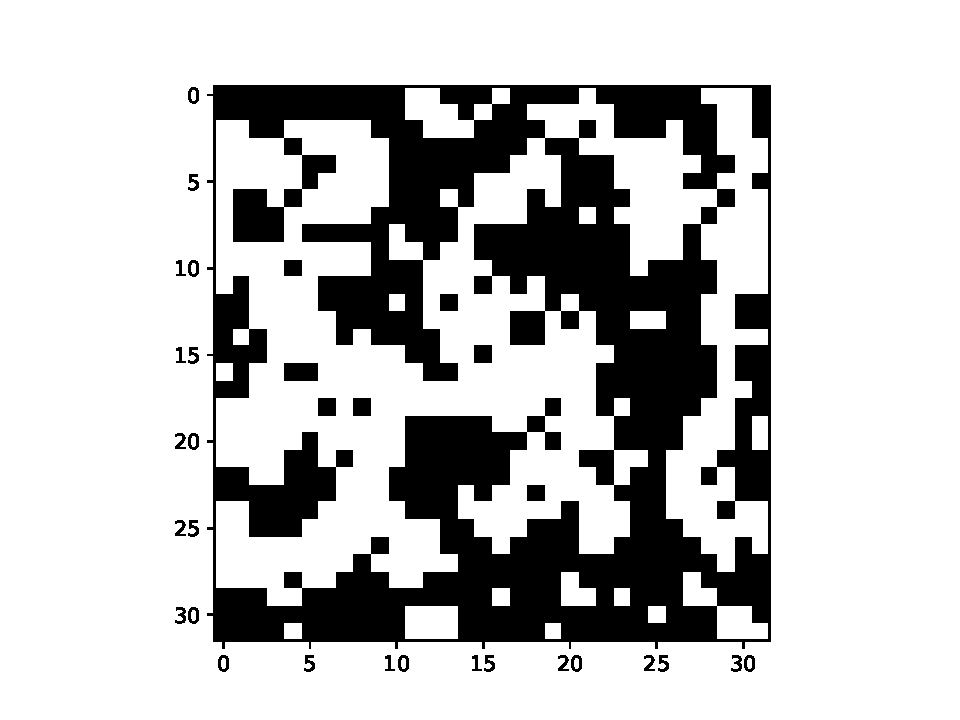
\includegraphics[scale=.5]{./figures/grid_1.5_0.pdf}
          }
        \end{minipage}%
        \begin{minipage}{.5\linewidth}
          \centering
          \subfloat[spins for $T=1.5$ after initialization]{
            \label{:b}
            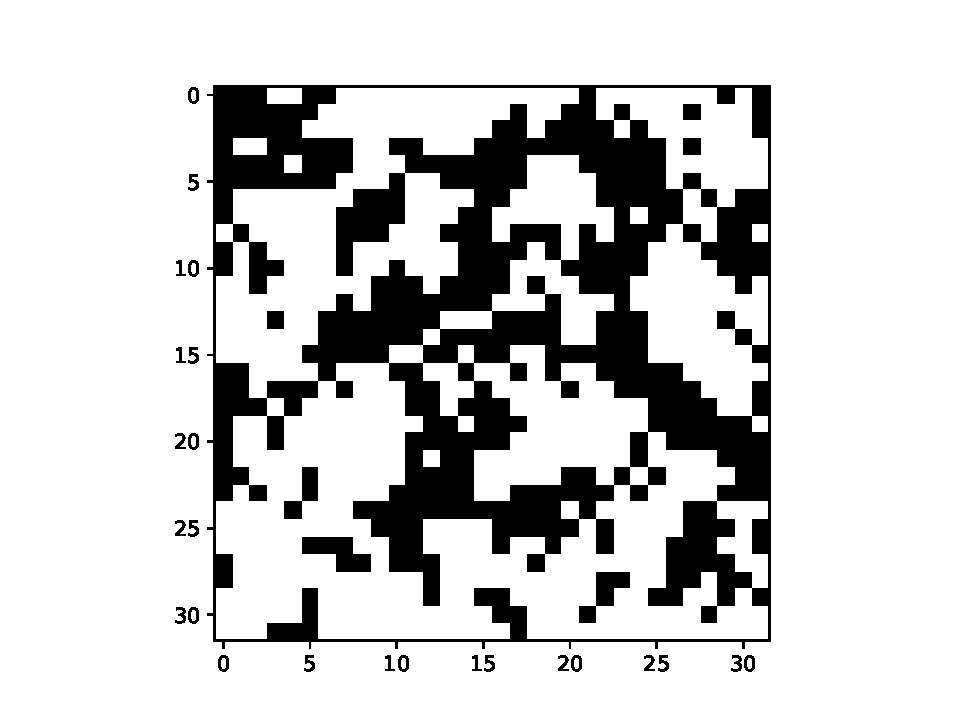
\includegraphics[scale=.5]{./figures/grid_3_0.pdf}
          }
        \end{minipage}
        \begin{minipage}{.5\linewidth}
          \centering
          \subfloat[spins for $T=1.5$ after 20 loops over the grid]{
            \label{:a}
            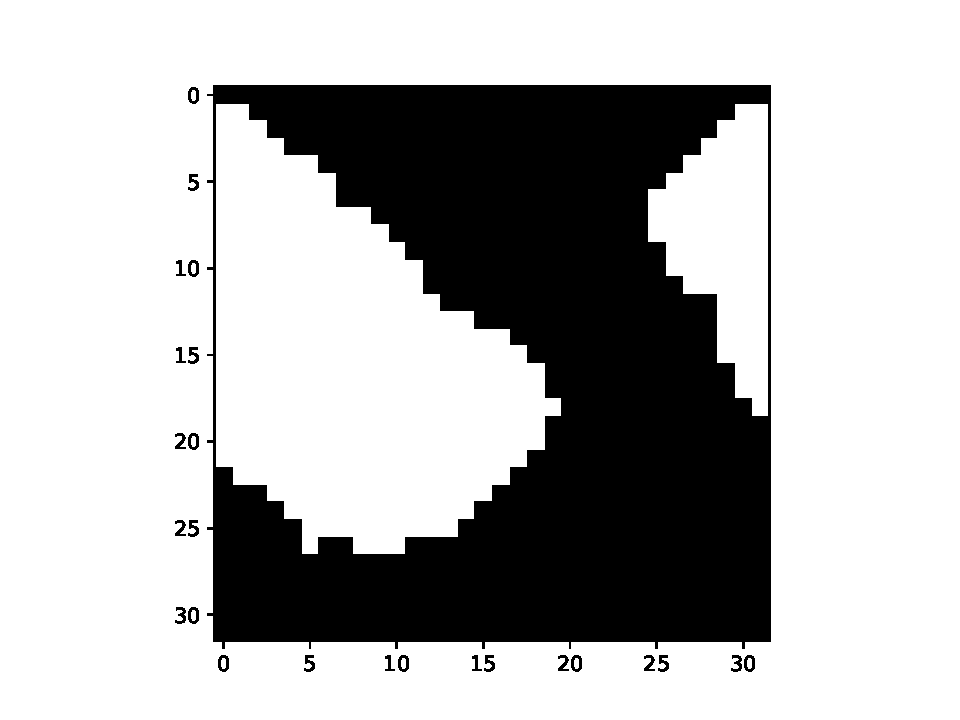
\includegraphics[scale=.5]{./figures/grid_1.5_20.pdf}
          }
        \end{minipage}%
        \begin{minipage}{.5\linewidth}
          \centering
          \subfloat[spins for $T=3$ after 20 loops over the grid]{
            \label{:b}
            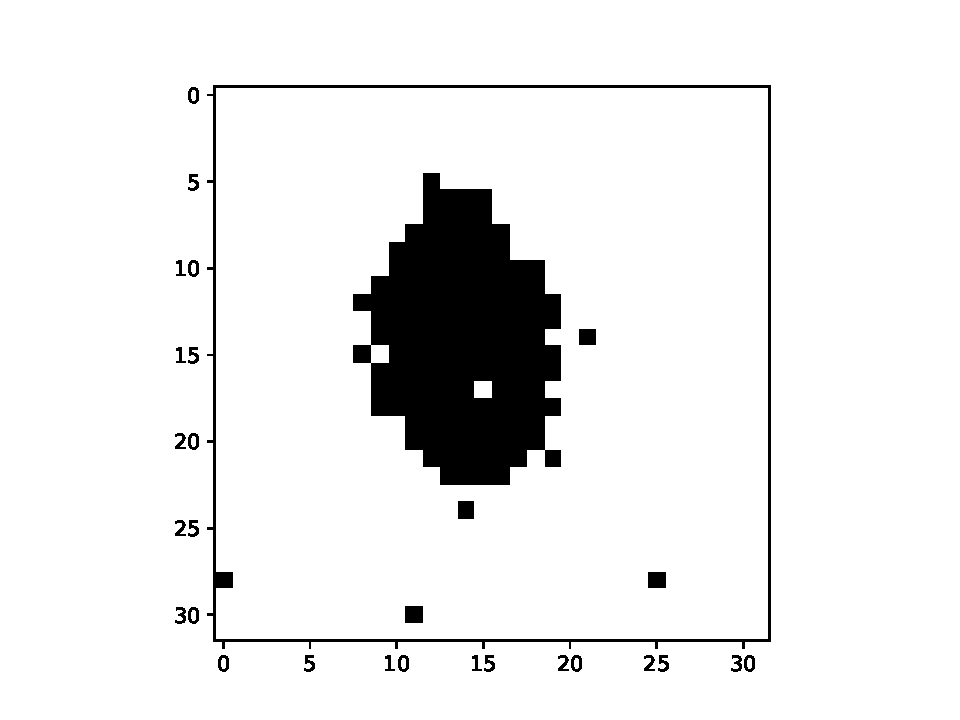
\includegraphics[scale=.5]{./figures/grid_3_20.pdf}
          }
        \end{minipage}
        \begin{minipage}{.5\linewidth}
          \centering
          \subfloat[spins for $T=1.5$ after 50 loops over the grid]{
            \label{:a}
            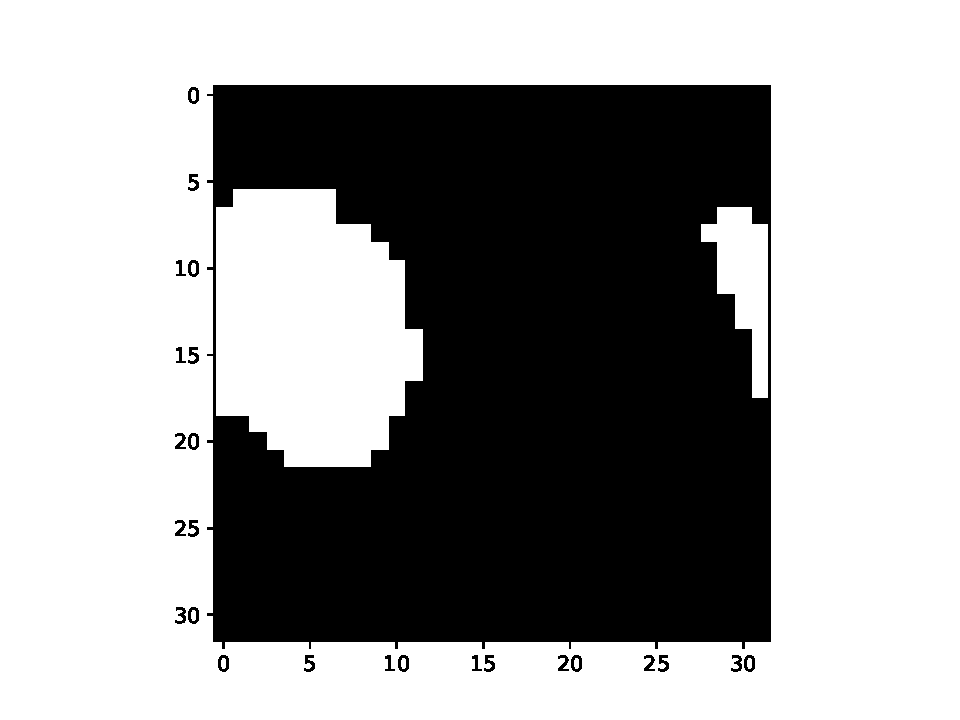
\includegraphics[scale=.5]{./figures/grid_1.5_50.pdf}
          }
        \end{minipage}%
        \begin{minipage}{.5\linewidth}
          \centering
          \subfloat[spins for $T=3$ after 50 loops over the grid]{
            \label{:b}
            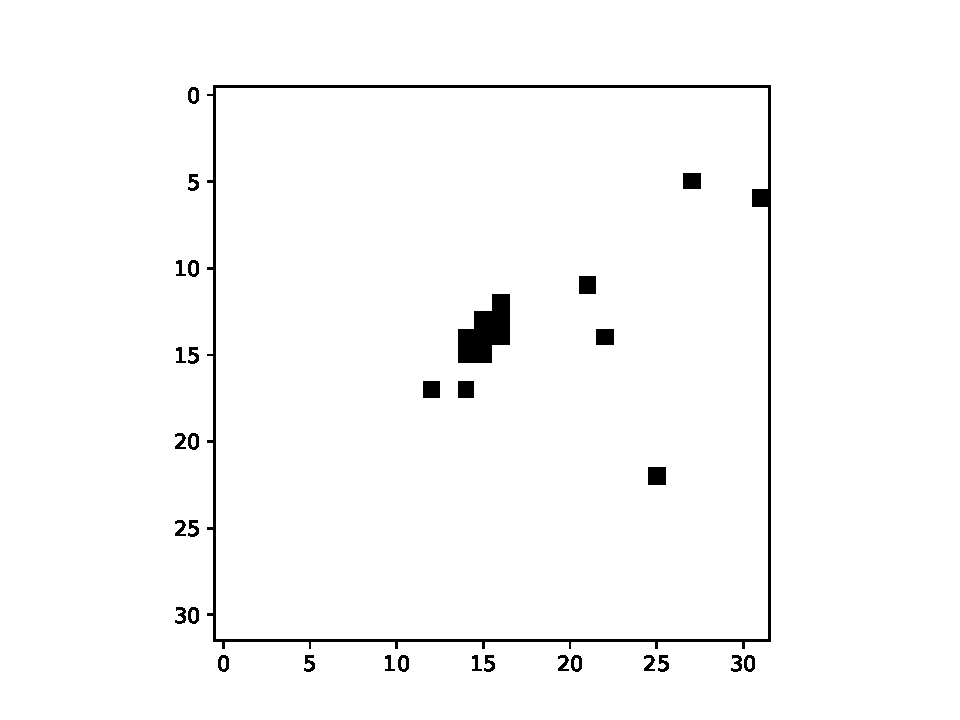
\includegraphics[scale=.5]{./figures/grid_3_50.pdf}
          }
        \end{minipage}

    \end{figure}
